\newpage
\section{Ricerca locale}
Gli agenti risolutori di problemi “classici” assumono: ambienti completamente osservabili, ambienti deterministici, sono nelle condizioni di produrre offline un piano
(una sequenza di azioni) che può essere eseguito senza imprevisti per raggiungere l’obiettivo.\\\\
La ricerca sistematica, o anche euristica, nello spazio di stati è troppo costosa. Inoltre spesso le assunzioni sull’ambiente sono da riconsiderare
infatti in ambienti realistizi le azioni sono non deterministiche e ambiente parzialmente osservabile oppure abbiamo addirittura ambienti sconosciuti e probemi di esplorazione (ess. ricerca online).\\\\
Per effetturare una \textbf{ricerca locale} bisogna fare alcune assunzione. Gli algoritmi visti esplorano gli spazi di ricerca alla ricerca di un goal e restituiscono un cammino soluzione,
ma a volte lo stato goal è la soluzione del problema. Gli algoritmi di ricerca locale sono adatti per problemi in cui:
\begin{itemize}
    \item La sequenza di azioni non è importante: quello che conta è unicamente lo stato goal.
    \item Tutti gli elementi della soluzione sono nello stato ma alcuni vincoli sono violati (Es. le regine nella formulazione a stato completo). Ci interessa di ottenere la soluzione ma non il path
\end{itemize}
Gli algoritmi di ricerca locale inoltre non sono sistematici, tengono traccia solo del nodo corrente e si spostano su nodi adiacenti. Non 
tengono traccia dei cammini (non servono in unscita!).
\begin{enumerate}
    \item Efficienti in occupazione di memoria.
    \item Possono trovare soluzioni ragionevoli anche in spazi molto grandi e inifini, come nel caso di spazi continui.
\end{enumerate}
Sono molto utili per risolvere probelmi di ottimazzione: lo stato migliore secondo una funzione obiettivo (f),
lo stato di costo minore (ma non il path).
\begin{example}
    Minimizare numero di regine sotto attacco (f all’obiettivo?) oppure training di un modello di Machine Learning.
\end{example}
\begin{figure}[h!]
    \centering
    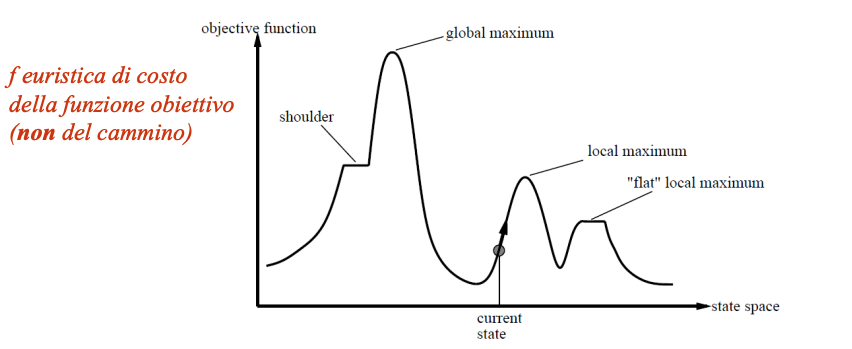
\includegraphics[width=0.7\textwidth]{images/panoram-spazio-stati.png}
\end{figure}
Uno stato ha una posizione sulla superficie e una altezza che corrisponde al valore della f. di valutazione (f. obiettivo).
Un algoritmo provoca movimento sulla superficie. Trovare l’avvallamento più basso (e.g. min costo) o il picco più alto (e.g. max di un obiettivo).

\subsection{Ricerca in salita (Hill climbing)}
È una ricerca locale di tipo \textbf{greedy}. Vengono generati i successori e valutati; viene scelto un nodo che migliora la valutazione dello stato attuale (non si tiene traccia degli altri [no albero di ricerca in memoria]).
\begin{itemize}
    \item Il migliore fra i sucessori è \textbf{Hill climbing a salita rapida/ripida}.
    \item Uno a caso (tra quelli che salgono) si dice \textbf{Hill climbing stocastico} (anche dipendendo da pendenza)
    \item Mentre il primo è il \textbf{Hill climbing con prima scelta} (il primo generato tra tanti possibili)
\end{itemize}
Se non ci sono stati successori migliori l’algoritmo termina con fallimento.
\begin{lstlisting}
    function Hill-climbing (problema)
        returns uno stato che e un massimo locale [esercizio: fare con min.]
        nodo-corrente = CreaNodo(problema.Stato-iniziale)
        
        loop do   
            vicino = il successore di nodo-corrente di valore piu alto
            if vicino.Valore <= nodo-corrente.Valore then
                return nodo-corrente.Stato // interrompe la ricerca
            nodo-corrente = vicino
            // (altrimenti, se vicino e migliore, continua)
\end{lstlisting}
\begin{note}
    Si prosegue solo se il vicino (più alto) è migliore dello stato corrente $\to$ se tutti i vicini sono peggiori o uguali si ferma.
\end{note}
Non c'è frontiera a cui ritornare, si tiene 1 solo stato. Il tempo si calcolo come numero di cicli variabile in base al punto di partenza.
Il codice in python è il seguente:
\begin{python}
    def hill_climbing(problem): """ Ricerca locale - Hill-climbing."""
        current = Node(problem.initial_state)
        while True:
            neighbors = [current.child_node(problem, action) for action in
                        problem.actions(current.state)]
            if not neighbors: 
                # se current non ha successori esci e restituisci current
                break

            # scegli il vicino con valore piu' alto (sulla funzione problem.value)
            neighbor = (sorted(neighbors,key = lambda x:problem.value(x), reverse = True))[0]
            if problem.value(neighbor) <= problem.value(current):
                break
            else:
                current = neighbor # (altrimenti, se vicino e migliore, continua)
        return current
\end{python}
\begin{example}
    Il problema delle 8 regine. Costo h (stima euristica del costo f): numero di coppie di regine che si attaccano a vicenda (nell'esempio valore 17).
    Si cerca il minimo, i numeri sono i valori dei successori (7x8) [7 posizioni per ogni regina, su ogni colonna], tra i migliori (di pari valore 12) si sceglie a caso,
    i imposta anche il minimo globale a 0.
    \begin{figure}[h!]
        \begin{subfigure}[b]{0.45\textwidth}
            \centering
            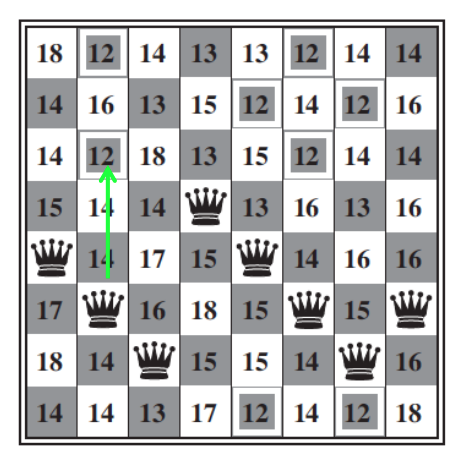
\includegraphics[width=\textwidth]{images/problema-8-regine.png}
        \end{subfigure}
        \begin{subfigure}[b]{0.45\textwidth}
            \centering
            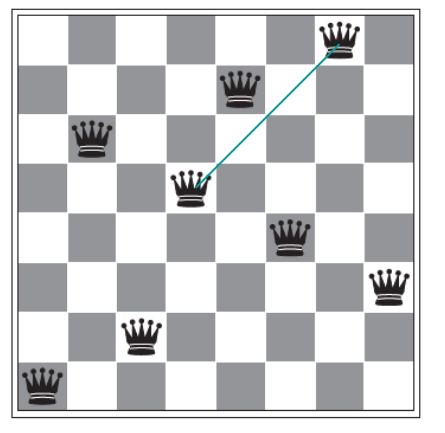
\includegraphics[width=\textwidth]{images/8-regine-esempio-negativo.png}
        \end{subfigure}
    \end{figure}
    \newpage
    Vediamo poi nella seconda figura un esempio negativo con minimo locale. Settiamo $h=1$, tutti gli stati successori non migliorano la situazione. 
    Per le 8 regine Hill-climbing si blocca l'$86\%$ delle volte, ma in media solo 4 passi per la soluzione e 3 quando si blocca, su $8^8 = 16.8$ milioni di stati. 
\end{example}
\begin{example}
    Sempre sulla stessa base dell'esempio sopra questo è un esempio positivo, con successo in tre mosse.
    \begin{figure}[h!]
        \centering
        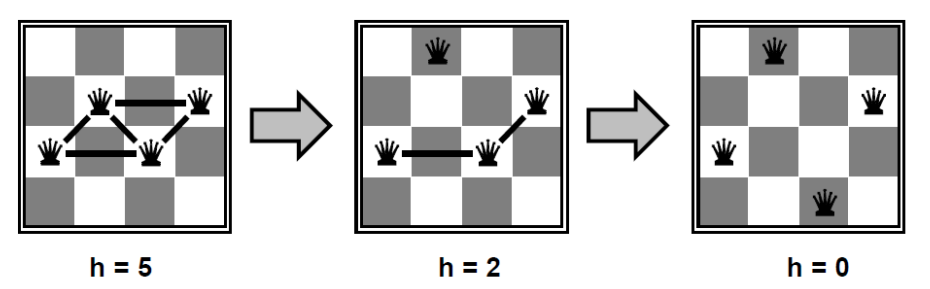
\includegraphics[width=0.7\textwidth]{images/8-regine-esempio-positivo.png}
    \end{figure}
    h qui è l'euristica di costo della funzione obiettico (da minimizzare).
\end{example}
Alcuni problemi con Hill-climbing ci sono se la f è da ottimizzare, infatti in questo caso i picchi sono massimi locali o soluzioni ottimali.
\begin{figure}[h!]
    \centering
    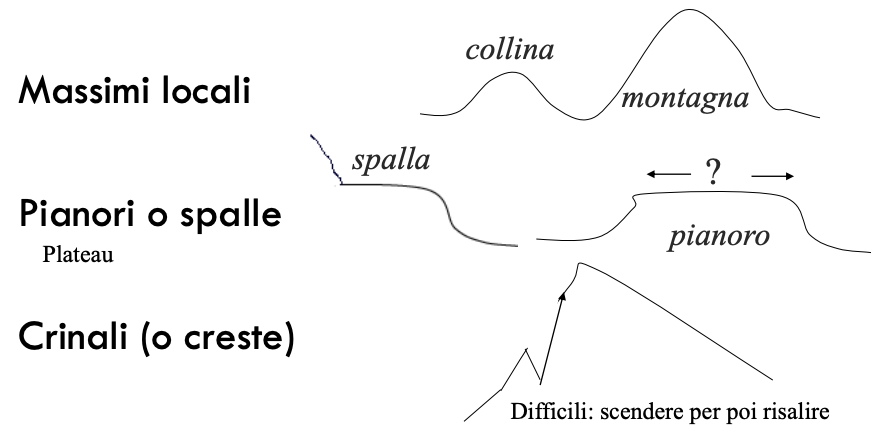
\includegraphics[width=0.75\textwidth]{images/problemi-hill-climbing.png}
\end{figure}

\hspace{-15pt}Alcuni miglioramenti che si possono apportare solo i seguenti:
\begin{enumerate}
    \item Consentire (un numero limitato di) mosse laterali (ossia ci si ferma per $<$ nell’alg. invece che per $\leq \to$ continua anche a parità di h). L’algoritmo sulle 8 regine ha successo nel $94\%$, ma impiega in media 21 passi.
    \item Hill-climbing stocastico: si sceglie a caso tra le mosse in salita (magari tenendo conto della pendenza). Converge più lentamente ma a volte trova soluzioni migliori.
    \item Hill-climbing con prima scelta. Può generare le mosse a caso, uno alla volta, fino a trovarne una migliore dello stato corrente (si prende solo il primo che migliora). Come la stocastica ma utile quando i successori sono molti (e.g. migliaia o ben oltre), evitando una scelta tra tutti.
    \item Hill-Climbing con riavvio casuale (random restart): ripartire da un punto scelto a caso. Se la probabilità di successo è p saranno necessarie in
    media 1/p ripartenze per trovare la soluzione (es. 8 regine, $p=0.14 \to 7$ ripartenze [1/p] per avere 6 fail e un successo). 
    Per le regine: caso con 3 milioni di regine in meno di un minuto! Se funziona o no dipende molto dalla forma del panorama degli stati (molti min loc. abbassano p, si blocca spesso)
\end{enumerate}

\subsection{Tempra simulata}
L’ algoritmo di tempra simulata (Simulated annealing) [Kirkpatrick, Gelatt, Vecchi 1983] combina hill-climbing con una scelta stocastica (ma non del tutto casuale, perché poco efficiente...).
Analogia con il processo di tempra dei metalli in metallurgia. I metalli vengono portati a temperature molto elevate (alta
energia/stocasticità iniziale) e raffreddati gradualmente consentendo di cristallizzare in uno stato a (più) bassa energia.
(esempio di cross-fertilization tra aree scientifche diverse).\\\\
In questo algoritmo ad ogni passo si sceglie un successore $n'$ a caso:
\begin{itemize}
    \item se migliora lo stato corrente viene espanso.
    \item se no (caso in cui $\Delta E = f(n') - f(n) \leq 0$) quel nodo viene scelto con probabilità $$p = e^{\Delta E/T} [0 \leq p \leq 1]$$ [Si genera un numero casuale tra 0 e 1: se questo è $<$ p il successore
    viene scelto, altrimenti no].
\end{itemize}
Ossia: p è inversamente proporzionale al peggioramento, infatti se la mossa peggiora molto, $\Delta E$ alto neg., la p si abbassa. 
T (temperatura) decresce col progredire dell’algoritmo (quindi anche p) secondo un piano definito. Col progredire rende improbabili le mosse peggiorative.\\\\
Per quanto riguarda l'analisi della tempra simulata, La probabilità p di una mossa in discesa diminuisce col tempo e l’algoritmo si comporta sempre di più come Hill Climbing.
Se T viene decrementato abbastanza lentamente con prob. tendentente ad 1 si raggiunge la soluzione ottimale. Analogia col processo di tempra dei metalli
T corrisponde alla temperatura $\Delta E$ alla variazione di energia.\\\\
I paramentri da inserire sono il valore iniziale e decremento di T, ed i valori 
per T determinati sperimentalmente: il valore iniziale di T è tale che per valori medi di $\Delta E, p=e^{\Delta E/T}$ sia all’incirca 0.5. 

\subsection{Ricerca local beam}
La versione locale della beam search. Si tengono in memoria k stati, anziché uno solo ed ad ogni passo si generano i successori di tutti i k stati
Se si trova un goal ci si ferma, altrimenti si prosegue con i k migliori tra questi
\begin{note}
    Diverso da K restart (che riparte da zero), diverso anche da beam search
\end{note}
\hspace{-15pt}Si introduce un elemento di casualità, come in un processo di selezione naturale (diversificare la nuova generazione).
Nella \textbf{variante stocastica} della local beam, si scelgono k successori, ma con probabilità maggiore per i migliori. Tra le terminolgie
usate abbiamo: organismo [stato], progenie [successori], fitness [il valore della f], idoneità.

\subsection{Algoritmi generici/evolutivi}
Sono varianti della beam search stocastica in cui gli stati successori sono ottenuti combinando due stati genitore (anziché per evoluzione).
Un po' di terminologia che si usera: \textbf{popolazione di individui} [stati], \textbf{fitness}, \textbf{accoppiamenti} + \textbf{mutazione genetica}, \textbf{generazioni}.\\\\
Allora per spiegare il funziomento vediamo insanzitutto che la \textbf{popolazione} iniziale è formata da:
\begin{itemize}
    \item k stati/\textbf{individui} generati casualmente.
    \item ogni individuo è rappresentato come una stringa (esempio: posizione nelle colonne (“24748552”) stato delle
    8 regine o con 24 bit*).
\end{itemize}
A questo punto gli individui sono valutati da una \textbf{funzione di fitness} (Esempio: n. di coppie di regine che non si attaccano).\\ 
Poi si \textbf{selezionano} gli individui per gli "\textbf{accoppiamenti}" con una probabilità proporzionale alla fitness.
Le coppie danno vita alla \textbf{generazione} successiva combinando materiale genetico (crossover) con un meccanismo aggiuntivo di mutazione genetica (casuale). 
La popolazione ottenuta dovrebbe essere migliore. La cosa si ripete fino ad ottenere stati abbastanza buoni (stati obiettivo) o finche non miglioriamo più.
\begin{example}
    \begin{figure}[h!]
        \centering
        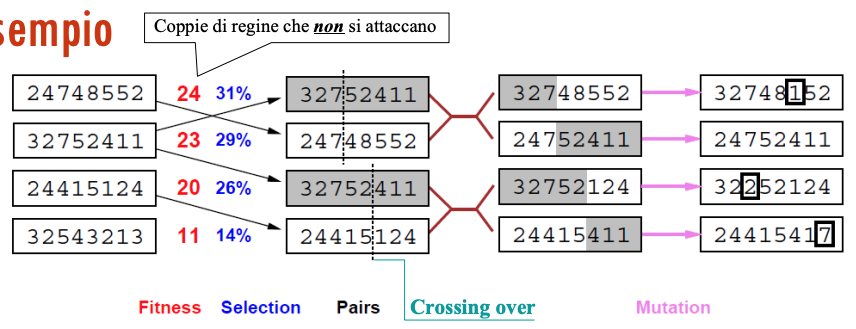
\includegraphics[width=0.8\textwidth]{images/esempio-algo-genetici.png}
    \end{figure}

    Per ogni coppia (scelta con probabilità(blu) proporzionale alla fitness(rosso)) viene scelto un punto di crossing over(verde) e vengono generati due figli scambiandosi pezzi (del DNA)
    Viene infine effettuata una mutazione(rosa) casuale che dà luogo alla prossima generazione,
    la fitness progressivamente tenderà a favorire generazioni migliori. Emula i meccanismi genetici ma anche l’evoluzione della specie.
    La nascita di un figlio aviene come:\\
    \begin{figure}[h!]
        \centering
        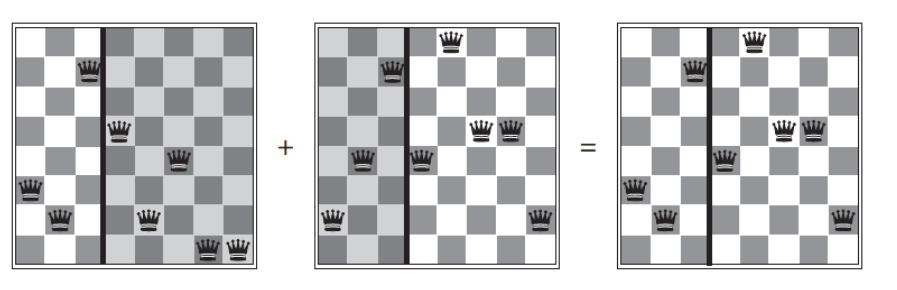
\includegraphics[width=0.75\textwidth]{images/nascita-figlio.png}
    \end{figure}

    \hspace{-15pt}Le parti chiare sono passate al figlio, le parti grigie si perdono, se i genitori sono molto diversi anche i nuovi stati sono diversi
    All'inizio spostamenti maggiori che poi si raffinano.
\end{example}
\hspace{-15pt}In conclusione gli algoritmi genetici sono suggestivi (area del Natural computing: e.g. swarm, ...). Usati in molti problemi reali e.g. configurazione di
circuiti e scheduling di lavori, fra i loro vantaggi abbiamo che combinano: tendenza a salire della beam search stocastica, interscambio info (indirettamente) tra thread paralleli di
ricerca (blocchi utili che si combinano). Funziona meglio se il problema (soluzioni) ha componenti significative rappresentate in sottostringhe.
Il maggior punto critico è la rappresentazione del problema in stringhe.

\subsection{Spazi continui}
Molti casi reali hanno spazi di ricerca continua e.g. fondamentale per Machine Learning! Stato descritto da variabili continue $x_1, \dots, x_n$, vettore x.
Prendiamo ad esemio movimenti in spazio 3D, con posizione data da $x = (x_1, x_2, x_3)$, apparentemente ostico, fattori di ramificazione infiniti con gli
approcci precedenti, in realtà molti strumenti matematici per spazi continui, che portano ad approcci anche molto efficienti...\\\\
Se la f è continua e differenziabile, e.g. quadratica rispetto a x (vettore). Il minimo o massimo si può cercare utilizzando il \textbf{gradiente}, che restituisce la
direzione di massima pendenza nel punto. Data f obiettivo su 3D
$$\nabla f = \Big ( \frac{\partial f}{\partial x_1}, \frac{\partial f}{\partial x_2}, \frac{\partial f}{\partial x_3} \Big)$$
Nell Hill climbing iterativo: $$x_{new} = x + \eta\nabla f(n)$$
Dove il '+' per salive (maximization), il '-' per scendere (minimization), la $\eta$ indica lo step size (e.g constante positiva $<$1)
\begin{figure}[h!]
    \centering
    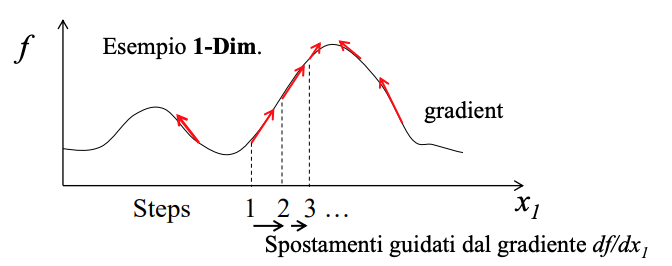
\includegraphics[width=0.65\textwidth]{images/spazi-continui-gradiant.png}
\end{figure}
Quantifica direzione e spostamento, senza cercarlo tra gli infiniti possibili successori!
\begin{note}
    non sempre è necessaio il min/max assoluto: vedremo nel ML
\end{note}
\begin{example}
    Discesa verso il minimo. $f(x) = x^2 \hspace{10pt} f'(x) = 2x$\\
    Discesa di gradiente verso il minimo. 
    $$x_{new} = x - \eta \nabla f(x) \to \:\:(1-d) \:\: \to x_{new} = x - \eta f'(x)$$
    Mettiamoci in $x=2$, la derivata vale $2 \times 2=4$, mi devo spostare di $-\eta f'(x) = -\eta4$, quindi ad esempio $(\eta = 0.2)$ ottengo $-\eta f'(x) = -0.2 \times 4 = -0.8$ andando a sinistra al punto $x_{new} = 2 - 0.8 = 1.2$ avvicinandomi quindi al minimo.
\end{example}

\subsection{Assunzioni sul'ambiente da considerare}
Negli ambienti più realistiti gli agenti risolutori di problemi “classici” assumono:
\begin{itemize}
    \item Ambienti completamente osservabili.
    \item Azioni/ambienti deterministici.
    \item Il piano generato è una sequenza di azioni che può essere generato offline e eseguito senza imprevisti.
    \item Le percezioni non servono se non nello stato iniziale.
\end{itemize}
In un ambiente parzialmente osservabile e non deterministico le \textbf{percezioni} sono importanti: restringono gli stati possibili, informano sull’effetto dell’azione.
Più che un piano l'agente può elaborare una "strategia", che tiene conto delle diverse eventualità: un \textbf{piano con contigenza}.
\begin{example}
    L'aspirapolvere con assunzioni diverse. \\
    L'spirapolvere imprevedibile: ci sono più stati possibili risulato dell'azione.
    \begin{itemize}
        \item Comportamento: Se aspira in una stanza sporca, la pulisce maa talvolta pulisce anche una stanza adiacente. Se aspira in una stanza pulita, a volte rilascia sporco.
        \item Variazioni necessarei al modello: Il modello di transizione restituisce un \textbf{insieme di stati}: l'agente non sa in quale si troverà. Il piano di \textbf{contingenza} sarà un piano condizionale e magari con cicli.
    \end{itemize}
    \begin{figure}[h!]
        \centering
        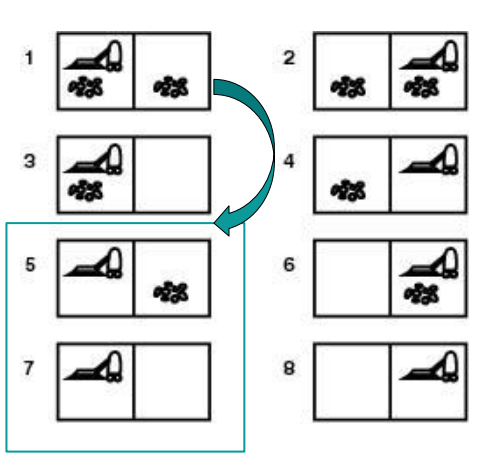
\includegraphics[width=0.34\textwidth]{images/esempio-aspirapolvere.png}
    \end{figure}
    \newpage
    Abbiamo che Risultati(aspira, 1) = $\{5, 7\}$. Il piano possibile potrebbe essere:
    \begin{lstlisting}
        Aspira, if stato = 5 
            then [Destra, Aspira]
            else []
    \end{lstlisting}
    La soluzione è da sequenza di azioni a piano (albero).
\end{example}
\subsubsection{Alberi di ricerca AND-OR}
\textbf{Nodi OR} le scelte dell’agente [1 sola azione]. \textbf{Nodi AND} le diverse contingenze (le scelte dell'ambiente, piu stati possibili), da considerare tutte.
Una soluzione a un problema di ricerca ANDOR è un albero che: ha un nodo obiettivo in ogni foglia specifica un’unica azione nei nodi OR include tutti gli archi uscenti da nodi AND (tutte le contingenze).
\begin{example}
    \begin{figure}[h!]
        \centering
        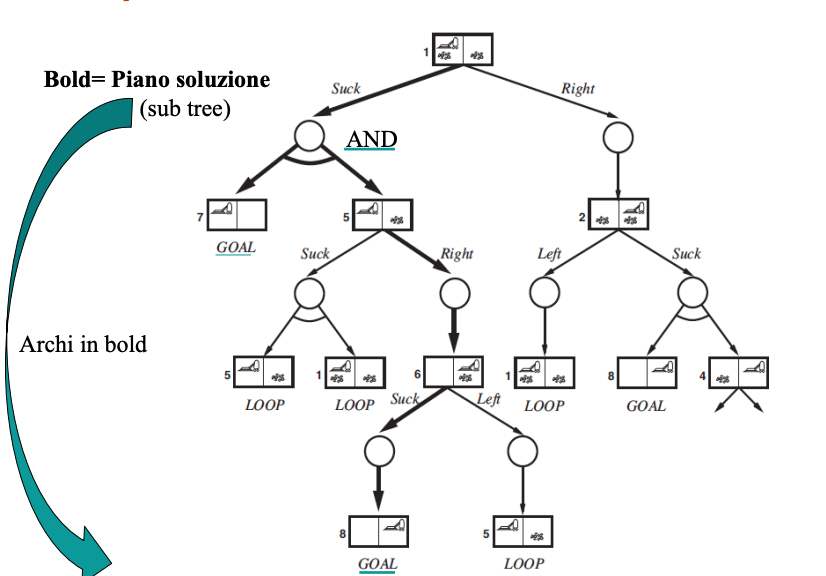
\includegraphics[width=0.75\textwidth]{images/esempio-and-or.png}
    \end{figure}
    Un piano di ricerca potrebbe essere il seguente:
    \begin{lstlisting}
        Aspira, if stato = 5 then [Destra, Aspira] else []
    \end{lstlisting}
\end{example}